\clearpage
\chapter{Grundlagen neuronaler Netze}
Im Rahmen dieses Kapitels werden die Grundlagen neuronaler Netze sowie die Convolutional Neural Networks (CNN) vermittelt.
Es werden die Aufgaben erklärt, die mithilfe dieser Netze gelöst werden und die in dieser Arbeit verwendete Netzarchitektur erläutert.

\section{Maschinelles Sehen}
\subsection{Objektdetektion}
Ziel der Objektdetektion ist es, das Vorhandensein von Objekten zu erkennen, ihre Position zu bestimmen und ihnen geeignete Klassenbezeichnungen zuzuordnen.
Diese Vorhersagen werden in der Regel durch eine Bounding Box dargestellt, die durch die Werte (x, y, Breite, Höhe) und die zugehörigen Klassenbezeichnungen definiert ist \cite{paperswithcode-compvis}.

\begin{figure}[h]
    \centering
    \includegraphics[width=.6\textwidth, angle=0]{img/22 nm_objectdetection.png}
    \label{fig:obdet}
    \caption{Messspitzen, die zur Lokalisierung und Differenzierung von Bounding Boxes umgeben sind. Quelle: Kleindiek Nanotechnik GmbH}
\end{figure}
\subsection{Instanz Segmentierung}
Die Instanz Segmentierung geht über die bloße Lokalisierung eines Objekts mit einer Bounding Box hinaus, indem jedem Pixel eine Klasse und Identifikationsnummer zugewiesen wird. Im Kontext der Spitzenerkennung ermöglicht dies die pixelgenaue Vorhersage, welche Bereiche des Bildes eine Spitze enthalten, sowie auch die Unterscheidung zwischen den einzelnen Spitzen. Jede Spitze erhält eine eindeutige Identifikation für genauere Analyse und Weiterverarbeitung \cite{paperswithcode-compvis}.
\begin{figure}[h]
    \centering
    \includegraphics[width=.6\textwidth, angle=0]{img/22 nm_instancesegmentation_nonum.png}
    \label{fig:inseg}
    \caption{Messspitzen, deren spezifische Formen durch Instanz Segmentierung hervorgehoben werden. Quelle: Kleindiek Nanotechnik GmbH}
\end{figure}
\subsection{Keypoint Erkennung}
Die Keypoint Erkennung identifiziert spezifische, markante Punkte von Objekten in einem Bild, die durch ihre x-y-Koordinaten definiert sind. Im Zusammenhang mit der Erkennung von Messspitzen ist der vorderste Punkt von besonderem Interesse, da er den direkten Kontakt mit der Probe herstellt und seine genaue Bestimmung wichtig ist \cite{paperswithcode-compvis}.
\begin{figure}[h]
    \centering
    \includegraphics[width=.6\textwidth, angle=0]{img/22 nm_keypoint_cross.png}
    \label{fig:keypdet}
    \caption{Messspitzen, deren vordere Punkte – die wesentlichen Kontaktpunkte bei der Probenmessung – deutlich markiert sind. Quelle: Kleindiek Nanotechnik GmbH}
\end{figure}
% \begin{figure}[ht]
%     \centering
%     \subfigure[]{\includegraphics[width=.32\textwidth, angle=0]{img/22 nm_objectdetection.png}}
%     \subfigure[]{\includegraphics[width=.32\textwidth, angle=0]{img/22 nm_instancesegmentation_nonum.png}}
%     \subfigure[]{\includegraphics[width=.32\textwidth, angle=0]{img/22 nm_keypoint_cross.png}}
%     \caption{Caption}
%     \label{fig:enter-label}
% \end{figure}
\clearpage
\section{Künstliche neuronale Netze}
In diesem Abschnitt werden der grundlegende Aufbau und die Funktionsweise von neuronalen Netzen sowie die verschiedenen Aktivierungsfunktionen, die bei den Berechnungen in den Netzen eine wichtige Rolle spielen, ausführlich beschrieben.
\subsection{Mehrschicht-Perzeptron}
\label{sec:mehrperz}
Wenn mehrere künstliche Neuronen schichtweise miteinander verbunden werden, ergibt sich ein mehrschichtiges Perzeptron \cite{RevModPhys.34.123}\cite{Rosenblatt.1958}. Es besteht aus mindestens drei Schichten, einer Eingabeschicht, einer oder mehrerer versteckten Schichten und einer Ausgabeschicht \cite{GARDNER19982627}. Die Schichten werden in der Regel voll verbunden. Das bedeutet, dass das Neuron einer Schicht eine Verbindung zu jedem Neuron der vorherigen oder nachfolgenden Schicht besitzt. Die Neuronen innerhalb einer Schicht sind dabei nicht miteinander verbunden. Da die Eingabe der Daten über eine einzelne Schicht erfolgt, werden die Daten zu einem eindimensionalen Array abgeflacht.
\begin{figure}[htbp]
\centerline{
\def\layersep{1.5cm}
\begin{tikzpicture}[
   shorten >=1pt,->,
   draw=black!50,
    node distance=\layersep,
    %every edge/.style={line width=2pt},
    every pin edge/.style={<-,shorten <=1pt, line width=2pt},
    neuron/.style={circle,fill=black!25,minimum size=17pt,inner sep=0pt},
    input neuron/.style={neuron, fill=green!50},
    output neuron/.style={neuron, fill=red!50},
    hidden neuron/.style={neuron, fill=blue!50},
    dotted neuron/.style={neuron, fill=black!50, dashed},
    annot/.style={text width=4em, text centered} ,
    xscale=1.5
]

    % Draw the input layer nodes
    \foreach \name / \y in {1,...,4}
        \node[input neuron, pin=left:$in_\y$] (I-\name) at (0,-\y) {};

    % Draw the hidden layer nodes
    \foreach \N in {1,2} {
       \foreach \y in {1,...,5} {
          \path[yshift=0.5cm]
              node[hidden neuron] (H\N-\y) at (\N*\layersep,-\y cm) {};
           }
    }

    % Draw the dotted layer nodes
    \foreach \y in {1,...,4}
        \node[dotted neuron] (D-\y) at (1.5*\layersep,-\y cm) {};

    % Draw the output layer nodes
    \foreach \y in {1,2}
        \node[output neuron,pin={[pin edge={->}]right:$out_\y$}, right of=H2-2, yshift=0.5cm-\y cm] (O-\y) {};

    % Connect every node in the input layer with every node in the hidden layer
    \foreach \source in {1,...,4}
        \foreach \dest in {1,...,5}
            \path (I-\source) edge[line width=2pt] (H1-\dest);

    % Connect every node in the hidden layer with every node in the dotted layer
    \foreach \source in {1,...,5}
        \foreach \dest in {1,...,4}
            \path (H1-\source) edge[dashed, line width=1.5pt] (D-\dest);

    % Connect every node in the dotted layer with every node in the next hidden layer
    \foreach \source in {1,...,4}
        \foreach \dest in {1,...,5}
            \path (D-\source) edge[dashed, line width=1.5pt] (H2-\dest);

    % Connect every node in the hidden layer with every node in the output layer
    \foreach \source in {1,...,5}
        \foreach \dest in {1,2}
            \path (H2-\source) edge[line width=2pt] (O-\dest);

    % Annotate the layers
    \node[annot,above of=I-1] {Input layer};
    \node[annot,above of=D-1, node distance=1.5cm, text width=6em] {Hidden layer};
    \node[annot,above of=O-1, node distance=2.5cm] {Output layer};
\end{tikzpicture}}
\caption{Ein mehrschichtiges Perzeptron mit 4 Eingängen und 2 Ausgängen. Zwischen Ein- und Ausgangsschacht liegen mehrere verborgene Schichten.}
\label{fig:multilp}
\end{figure}
Dies birgt den Vorteil, dass das mehrschichtige Perzeptron nicht durch die Form der Daten beschränkt ist. Allerdings gehen dadurch räumliche Informationen verloren, die für die Bildverarbeitung fundamental sind. Dieses Problem wird durch das CNN gelöst, das in Abschnitt \ref{sec:convnet} beschrieben wird.

Die folgenden versteckten Schichten sind für die Erkennung und Modellierung komplexer Zusammenhänge in den Eingabedaten. Ihre Anzahl wirkt sich auf die Lernfähigkeit, die Komplexität und die Generalisierungsfähigkeit des Modells aus und variiert je nach Komplexität des zu lösenden Problems und der Größe der verfügbaren Daten. Werden viele versteckte Schichten verwendet, spricht man von einem tiefen neuronalen Netz.

Die Ausgabeschicht ist die letzte Schicht des Netzwerkes und hat die Aufgabe, die Ergebnisse des Netzes in einer für das Problem geeigneten Form darzustellen. Sie besteht aus einer Anzahl von Neuronen, die der Anzahl der gewünschten Ausgabewerte entspricht.

\subsection{Aktivierungsfunktion}
Die Aktivierungsfunktion ist ein wesentlicher Bestandteil von künstlichen neuronalen Netzen. Sie wird auf die Summe der gewichteten Eingaben eines jeden Neurons angewendet und generiert die Ausgabe.

Die Nichtlinearität der Funktion ist dabei von entscheidender Bedeutung. Sie ermöglicht dem neuronalen Netz die Modellierung komplexer Muster und Beziehungen in den Daten und damit die Approximation komplexer Funktionen. Ohne die Nutzung einer Aktivierungsfunktion, würde das Netzwerk nur lineare Transformationen durchführen, was die Generalisierungsfähigkeit stark einschränken würde. Einige Aktivierungsfunktionen haben einen Schwellenwert, bei deren Überschreitung sie aktiviert werden und einen entsprechenden Ausgabewert erzeugen. Wichtige Aktivierungsfunktionen sind die Sigmoidfunktion, die ReLU-Funktion (Rectified Linear Unit) und die Tanh-Funktion (Hyperbolischer Tangens) \cite{APICELLA202114}.

\begin{figure}[h]
    \centering
    \subfigure[Binäre Stufenfunktion]{
    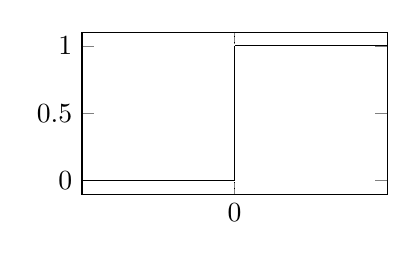
\begin{tikzpicture}
    	\begin{axis}[xmin=-5,xmax=5,xtick={0},xticklabels={0},height=0.3*\textwidth,width=0.45*\textwidth]
    		\addplot[domain=-5:0] {0};
            \addplot[domain=0:5] {1};
            \draw (axis cs:0,0) -- (axis cs:0,1);
            \draw[dotted] (axis cs:0,-1) -- (axis cs:0,2);
    	\end{axis}
    \end{tikzpicture}
    \label{fig:schwelle}
    }
    \subfigure[Sigmoid]{
    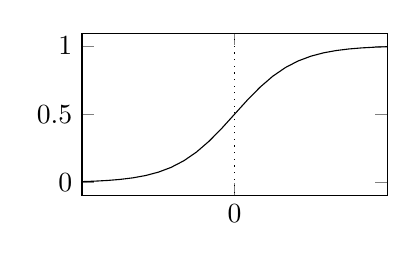
\begin{tikzpicture}
    	\begin{axis}[xmin=-5,xmax=5,xtick={0},xticklabels={0},height=0.3*\textwidth,width=0.45*\textwidth]
    		\addplot[] {1/(1+e^-x)};
            \draw[dotted] (axis cs:0,-1) -- (axis cs:0,2);
    	\end{axis}
    \end{tikzpicture}
    \label{fig:sigmoid}
    }\\\;\;
    \subfigure[ReLU]{
    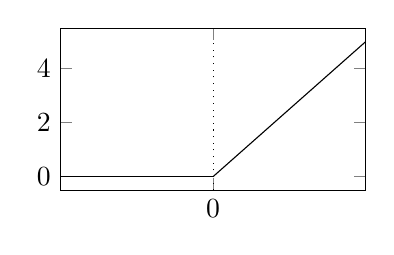
\begin{tikzpicture}
    	\begin{axis}[xmin=-5,xmax=5,xtick={0},xticklabels={0},height=0.3*\textwidth,width=0.45*\textwidth]
    		\addplot[domain=-5:0] {0};
            \addplot[domain=0:5] {x};
            \draw[dotted] (axis cs:0,-1) -- (axis cs:0,5);
    	\end{axis}
    \end{tikzpicture}
    \label{fig:relu}
    }
    \subfigure[Tanh]{
    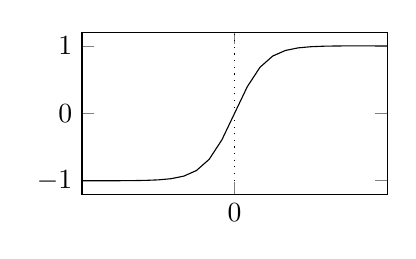
\begin{tikzpicture}
    	\begin{axis}[xmin=-5,xmax=5,xtick={0},xticklabels={0},height=0.3*\textwidth,width=0.45*\textwidth]
    		\addplot[domain=-5:5] {tanh(x)};
            \draw[dotted] (axis cs:0,-1) -- (axis cs:0,5);
    	\end{axis}
    \end{tikzpicture}
    \label{fig:tanh}
    }
    \caption{Graphen der Binären Stufen-, Sigmoid- und ReLU-Funktion}
    \label{fig:aktfunk}
\end{figure}
Die Sigmoidfunktion (siehe \ref{fig:sigmoid}) nimmt einen beliebigen Eingabewert und wandelt ihn in einen Ausgabewert zwischen 0 und 1 um. Sie ist besonders nützlich in der Ausgabeschicht von Klassifikationsproblemen, bei denen die Ausgabe eine Wahrscheinlichkeit ist.
Die Tanh-Funktion (dargestellt in \ref{fig:tanh}) wandelt, ähnlich wie die Sigmoid-Funktion, jeden Eingabewert in einen Ausgabewert zwischen -1 und 1 um, was sie nützlicher für Ausgaben macht, die sowohl positive als auch negative Werte annehmen sollen.
Im Gegensatz dazu gibt die ReLU-Funktion (vgl. \ref{fig:relu}) den Eingabewert unverändert zurück, wenn er positiv ist, und Null, wenn er negativ ist. Ein wesentlicher Vorteil der ReLU-Funktion ist, dass sie das Problem des verschwindenden Gradienten – bei dem die tiefen Schichten des Netzes nicht lernen – vermeidet, das bei älteren Aktivierungsfunktionen wie Tanh und Sigmoid auftritt \cite{atoum2023adaptive}. Außerdem hat sie einen geringeren Rechenaufwand.

Jede dieser Aktivierungsfunktionen hat ihre eigenen Eigenschaften und Verwendungszwecke, und die Wahl der richtigen Funktion hängt von dem spezifischen Problem und den Eigenschaften der Daten ab. In der Praxis werden häufig verschiedene Aktivierungsfunktionen in verschiedenen Schichten eines neuronalen Netzes verwendet, um die Leistung zu optimieren.
\section{Convolutional Neural Networks}
\label{sec:convnet}
CNNs sind eine Form künstlicher neuronaler Netze, die speziell für die Verarbeitung und Extraktion räumlicher Informationen aus Daten, insbesondere aus Bildern und anderen mehrdimensionalen Datenstrukturen, entwickelt wurden \cite{8308186}.
Sie sind ein wichtiger Bestandteil in vielen modernen maschinellen Lernsystemen, insbesondere im Bereich des maschinellen Sehens und haben wesentlich dazu beigetragen, die Leistungsfähigkeit von Algorithmen in Aufgaben wie Bild- und Videoklassifikation, Objekterkennung und Segmentierung zu verbessern \cite{oshea2015introduction}.

Das grundlegende Prinzip eines CNN besteht darin, kleine, lokalisierte Merkmale aus den Eingabedaten zu lernen und diese dann zu abstrahieren und zu kombinieren, um komplexere Muster und Strukturen zu erkennen. Ein CNN besteht typischerweise aus drei Arten von Schichten: Convolution-Schichten (Abbildung \ref{sec:conv}), Pooling-Schichten (dargestellt in \ref{sec:pool}) und Fully Connected-Schichten, die einem mehrschichtigen Perzeptron (Erklärung in \ref{sec:mehrperz}) ähnlich sind.

\subsection{Convolution-Schichten}
\label{sec:conv}
Convolution-Schichten sind entscheidend für die Extraktion von Merkmalen aus den Eingabedaten. Im Folgenden wird die Arbeitsweise näher erläutert.

In einer Faltungsschicht wird ein Filter – auch Kernel genannt –, der aus einer Matrix von Gewichten besteht, über die gesamte Eingabe geschoben. Dieser Vorgang wird als Convolution (Faltung) bezeichnet und ist in Abbildung \ref{fig:conv} dargestellt. Klassische Filtergrößen sind dabei 3×3, 5×5 oder 7×7. Die Filter sind daher in der Regel viel kleiner als die Eingabe, decken aber die gesamte Tiefe der Eingabe ab. Bei einem Farbbild beträgt die Tiefe beispielsweise drei.

Durch die Anwendung dieser Filter auf die Eingabedaten, identifizieren die\\Convolution-Schichten Muster, Kanten und Texturmerkmale. Die Simulation des Verschiebens der Filter über die Eingabedaten wird durch sogenannte rezeptive Felder simuliert. Dabei werden die Neuronen einer Schicht ausschließlich mit den Neuronen der vorhergehenden Schicht verbunden, die innerhalb des durch die Filtergröße definierten rezeptiven Feldes liegen. Diese lokale Verknüpfung ermöglicht es dem CNN, räumliche Informationen zu erfassen und lokal relevante Merkmale zu extrahieren, während gleichzeitig die Anzahl der zu lernenden Parameter durch die gemeinsame Nutzung von Parametern (da der Filter auf mehrere Bereiche des Bildes angewendet wird) reduziert wird \cite{weisstein_convolution}.

Um die Ausgabegröße der Convolution-Schichten zu steuern und sicherzustellen, dass sie genügend räumliche Information enthalten, können zwei wichtige Parameter verwendet werden: Padding und Stride.

\begin{figure}[htbp]
    \centering
    %\vspace{3cm}
    \begin{tikzpicture}[]%[scale = 0.7, transform canvas={scale=0.7}]
      % Padded input matrix
      \matrix (input) [matrix of nodes, nodes={draw, minimum size=.85cm}] {
        0 & 0 & 0 & 0 & 0 \\
        0 & 1 & 2 & 3 & 0 \\
        0 & 4 & 5 & 6 & 0 \\
        0 & 7 & 8 & 9 & 0 \\
        0 & 0 & 0 & 0 & 0 \\
      };
      % Kernel matrix
      \matrix (kernel) [right=2cm of input.north east, matrix of nodes, nodes={draw, minimum size=0.6cm}] {
        1 & 0 & -1\\
        2 & 0 & -2\\
        1 & 0 & -1\\
      };
      % Convolved matrix (with padding)
      \matrix (conv) [right=6cm of input, matrix of nodes, nodes={draw, minimum size=.88cm}] {
        -9 & -9 & 9 \\
        -20 & -8 & 20 \\
        -21 & -6 & 21 \\
      };
      % Labels
      \node[above=1ex of input, font=\large] {Padded Input};
      \node[above=1ex of kernel, font=\large] {Kernel};
      \node[above=1ex of conv, font=\large] {Output};
    
      % Convolution operation
      \begin{scope}[thick, red, on background layer]
        \node[draw, thick, fill=red!30, fit={(input-1-1) (input-3-3)}, inner sep=0pt] (box1) {};
        \node[draw, thick, red, fit={(kernel-1-1) (kernel-3-3)}, inner sep=0pt] (box2) {};
        \node[draw, thick, fill=red!30, fit={(conv-1-1) (conv-1-1)}, inner sep=0pt] (box3) {};
        \draw[thick, ->] (box1) -- (box2);
        \draw[thick, ->] (box2) -- (conv-1-1);
      \end{scope}
    \end{tikzpicture}
    %\hspace{5cm}
    %\vspace{2cm}
    \caption{Zero-padded Bild. Der Stride ist eins. Somit entspricht die Ausgangsgröße der Faltung der Eingangsgröße. Der Sobel-Operator wird als Kernel verwendet \cite{kanopoulos1988design}.}
    \label{fig:conv}
\end{figure}
Padding bezieht sich auf das Hinzufügen zusätzlicher Randpixel zur Eingabe, bevor der Filter angewendet wird. Dadurch wird sichergestellt, dass die Größe der Ausgabe erhalten bleibt, insbesondere wenn der Filter über die Ränder der Eingabe gleitet \cite{convolution}.

Stride bezieht sich auf die Anzahl der Pixel, um die der Filter bei jedem Schritt über die Eingabe gleitet. Ein Stride von eins bedeutet, dass der Filter Pixelweise verschoben wird, während ein größerer Stride zu größeren Schritten führt. Ein größerer Stride reduziert die räumliche Dimension der Ausgabe, da weniger Positionen des Filters überprüft werden. Dadurch kann die Größe der Netzarchitektur reduziert werden \cite{convolution}.

\subsubsection{Dilated-Convolution}
\label{sec:dilconv}
Dilated Convolution, auch bekannt als Atrous Convolution, ist eine von Yu \textit{et al.} entwickelte Technik zur effektiven Erweiterung des Rezeptiven Feldes in einer CNN-Architektur, ohne dabei die räumliche Auflösung zu verlieren oder die Anzahl der Parameter zu erhöhen \cite{yu2015multi}.
\begin{figure}[htbp]
    \centering
    \includegraphics[width=.7\linewidth]{img/dilconv.png}
    \captionsource{(a) 1-dilated convolution mit 3x3 rezeptivem Feld, (b) 2-dilated convolution mit 7x7 rezeptivem Feld, (c) 4-dilated convolution mit 15x15 rezeptivem Feld}{Dilated Residual Networks \cite{Yu_2017_CVPR}}
    \label{fig:dilconv}
\end{figure}
Die Technik verwendet eine sogenannte Verdünnungsrate (dilation rate), die die Abstände zwischen den Gewichten in der Filtermaske vergrößert. Ein Beispiel ist in Abbildung \ref{fig:dilconv} dargestellt. Durch die Anwendung von Dilated-Convolutions kann das Netz somit mehr Kontextinformation aus dem Eingabebild extrahieren, ohne die Komplexität des Netzes wesentlich zu erhöhen. Yu \textit{et al.} zeigen, dass diese Technik besonders wertvoll in Anwendungen ist, die eine detaillierte Segmentierung erfordern, da sie es ermöglicht, Informationen über größere Eingangsbereiche zu sammeln und gleichzeitig eine hohe Auflösung in der Ausgabe beizubehalten \cite{Yu_2017_CVPR}. Insbesondere bei Aufgaben, bei denen es auf die genaue Lokalisierung von Objekten ankommt, wie beispielsweise der Spitzenerkennung in Nanoprobing-Anwendungen, kann der Einsatz von Dilated-Convolutions zu verbesserten Ergebnissen führen.

\subsection{Pooling-Schichten}
\label{sec:pool}
Pooling-Schichten bilden einen weiteren wichtigen Bestandteil von CNNs, sie werden dazu genutzt, die Dimension der von Convolution-Schichten erzeugten Featuremaps zu reduzieren und gleichzeitig wichtige Merkmale beizubehalten \cite{pooling}. Dies wird erreicht, indem benachbarte Werte über eine Funktion reduziert werden. Die häufigsten Pooling-Operationen sind das Max-Pooling und das Average-Pooling.\\
\begin{figure}[htbp]
    \centering
    \vspace{0cm}
    \begin{tikzpicture}[]%[scale = 0.7, transform canvas={scale=0.7}]
      % Input matrix
      \matrix (input) [matrix of nodes, nodes={draw, minimum size=.8cm}] {
        7 & 3 & 9 & 1 \\
        4 & 6 & 2 & 8 \\
        2 & 5 & 7 & 3 \\
        8 & 1 & 5 & 9 \\
      };
      % Max-Pooled matrix
      \matrix (maxpooled) [above right=2cm of input.east, matrix of nodes, nodes={draw, minimum size=.8cm}] {
        7 & 9 \\
        8 & 9 \\
      };
    
      % Pooled matrix
      \matrix (avgpooled) [below right=2cm of input.east, matrix of nodes, nodes={draw, minimum size=.8cm}] {
        5 & 5 \\
        4 & 6 \\
      };
      
      % Labels
      \node[above=1ex of input, font=\large] {Input};
      \node[above=1ex of maxpooled, font=\large] {Max Pooled};
      \node[above=1ex of avgpooled, font=\large] {Average Pooled};
    
      % Pooling operation
      \begin{scope}[thick, red, on background layer]
        \node[draw, thick, fill=red!30, fit={(input-1-1) (input-2-2)}, inner sep=0pt] (box1) {};
        \node[draw, thick, fill=red!30, fit={(maxpooled-1-1)}, inner sep=0pt] (box2) {};
        \node[draw, thick, fill=red!30, fit={(avgpooled-1-1)}, inner sep=0pt] (box8) {};
        
        \node[draw, thick, fill=yellow!30, fit={(input-1-3) (input-2-4)}, inner sep=0pt] (box3) {};
        \node[draw, thick, fill=yellow!30, fit={(maxpooled-1-2)}, inner sep=0pt] (box4) {};
        \node[draw, thick, fill=yellow!30, fit={(avgpooled-1-2)}, inner sep=0pt] (box9) {};
        
        \node[draw, thick, fill=blue!30, fit={(input-3-1) (input-4-2)}, inner sep=0pt] (box4) {};
        \node[draw, thick, fill=blue!30, fit={(maxpooled-2-1)}, inner sep=0pt] (box5) {};
        \node[draw, thick, fill=blue!30, fit={(avgpooled-2-1)}, inner sep=0pt] (box10) {};
        
        \node[draw, thick, fill=green!30, fit={(input-3-3) (input-4-4)}, inner sep=0pt] (box6) {};
        \node[draw, thick, fill=green!30, fit={(maxpooled-2-2)}, inner sep=0pt] (box7) {};
        \node[draw, thick, fill=green!30, fit={(avgpooled-2-2)}, inner sep=0pt] (box11) {};
      \end{scope}
      \draw[thick, ->] (box1) -- (box2);
      \draw[thick, ->] (box1) -- (box8);
    \end{tikzpicture}
    \hspace{0cm}
    \vspace{0cm}
    \caption{Pooling dient der Dimensionsreduktion unter Beibehaltung der aussagekräftigsten Merkmale, wobei Methoden wie Max-Pooling und Average-Pooling zum Einsatz kommen.}
    \label{fig:pad}
\end{figure}
Beim Max-Pooling wird in jedem Pooling-Bereich der maximale Wert als repräsentativer Wert verwendet. Dies hilft dabei, herausragende Merkmale oder Aktivierungen hervorzuheben und die Positionsinformationen zu erhalten.
Beim Average-Pooling wird hingegen der Durchschnitt der Werte im Pooling-Bereich berechnet. Dadurch werden die Werte geglättet und das Netzwerk wird robuster gegenüber kleinen lokalen Verschiebungen.
Über die Kernelgröße, den Stride und das Padding kann die Ausgabegröße der Pooling-Schicht wie bei der Convolution bestimmt werden.
\clearpage
\section{Mask R-CNN}
Mask R-CNN ist ein innovativer Ansatz für Instanzsegmentierungsaufgaben, der auf dem Konzept der Region Based Convolutional Neural Networks (R-CNNs) basiert \cite{Girshick_2015_ICCV}\cite{7112511}. Mask R-CNN wurde 2017 von He \textit{et al.} bei Facebook AI Research entwickelt und erstmals veröffentlicht \cite{He_2017_ICCV}. Es stellt einen Meilenstein in der Entwicklung von Algorithmen zur Objekterkennung und -segmentierung dar.
Mask R-CNN erweitert und verbessert das von Ren \textit{et al.} entwickelte Modell Faster R-CNN \cite{DBLP:journals/corr/RenHG015} in mehreren Punkten.
\begin{figure}[htbp]
    \centering
    \includegraphics[width=\linewidth]{img/maskrcnn_network_custom.png}
    \captionsource{Mask R-CNN Architektur}{Modifiziert aus der MathWorks Dokumentation \cite{mathworks-maskrcnn}}
    \label{fig:maskrcnn}
\end{figure}
Dem Modell wird ein zusätzlicher Segmentierungszweig hinzugefügt, der es ermöglicht, für jedes erkannte Objekt eine präzise, pixelgenaue Maske zu erzeugen. Diese Eigenschaft unterscheidet Mask R-CNN von Faster R-CNN und erweitert dessen Fähigkeiten über die reine Objekterkennung und -klassifikation hinaus. Darüber hinaus implementiert Mask R-CNN eine sogenannte RoIAlign Schicht, um das Problem der Diskrepanz zwischen dem RoIPooling in Faster R-CNN und der pixelgenauen Segmentierung zu lösen, was zu einer weiteren Verbesserung der Modellleistung führt. Die Implementierung von RoIAlign wird im Rahmen dieser Arbeit nicht weiter behandelt und kann in dem von He \textit{et al.} veröffentlichten Paper \cite{He_2017_ICCV} entnommen werden.
\subsection{Backbone Netzwerk}
\label{sec:backbone}
Das Backbone-Netz wird verwendet, um tief abstrahierte Merkmale aus den Eingabedaten zu extrahieren. Es stellt die erste Stufe von Mask R-CNN dar. In Abbildung \ref{fig:maskrcnn} ist sie als \glqq CNN\grqq{} linken dargestellt.
Die extrahierten Merkmale dienen als Input für den Rest des Netzes, das spezifische Aufgaben wie Objekterkennung, Segmentierung oder Klassifikation durchführt.
Die Wahl des Backbone-Netzes hat einen wesentlichen Einfluss auf die Leistungsfähigkeit des Gesamtsystems. Sie hängt von der Komplexität des Problems, den spezifischen Anforderungen der Aufgabe und der Rechenkapazität ab.

Residuale Netzwerke (ResNet) welche erstmal von He \textit{et al.} vorgestellt wurden \cite{He_2016_CVPR}, lösen das Problem des vanishing/exploding Gradienten \cite{7112511} in tiefen Netzen durch die Nutzung von skip-connections \cite{1603.05027}\cite{1701.09175}\cite{1507.06228}. Sie sind eine weit verbreitete Wahl für die Objektdetektion und -segmentierung \cite{2206.08016}.
ResNets gibt es in verschiedenen Tiefen, darunter Modelle wie ResNet-50 und ResNet-101, wobei sich jede Zahl auf die Anzahl der Convolution-Schichten im Netzwerk bezieht. Tiefere Modelle können in der Regel komplexere Merkmale erfassen, benötigen jedoch mehr Rechenleistung und Speicherplatz.

\begin{figure}[htbp]
    \centering
    \includegraphics[width=\linewidth, angle=180]{img/resnet34.png}
    \captionsource{Architektur des ResNet-34. ResNet Netze bestehen aus mehreren Ebenen. Jede Ebene extrahiert Merkmale auf einer anderen Abstraktionsebene.}{\cite{He_2016_CVPR}}
    \label{fig:resnet34}
\end{figure}
ResNet-FPN, wobei FPN für Feature Pyramid Network steht, ist eine Variante des ResNet-Modells, die speziell für Aufgaben entwickelt wurde, die eine Objekterkennung auf unterschiedlichen Skalen erfordern. Ein FPN verbessert die Fähigkeit von ResNets, Objekte unterschiedlicher Größe zu erkennen, indem eine Pyramide von Feature-Maps erzeugt wird, die von der hochauflösenden, semantisch schwachen Ebene bis zur niedrigauflösenden, semantisch starken Ebene reicht. Für weitere Informationen zu FPN siehe \cite{1612.03144}.

Eine weitere für diese Arbeit relevante Variante der ResNet-Architektur ist ResNet-DC5. Diese Konfiguration enthält – anstelle von FPN – Dilated Convolutions \ref{sec:dilconv} in der C5-Ebene von ResNet. Die Integration von Dilated Convolutions ermöglicht es dem Netzwerk, mehr Kontextinformationen aus dem Eingabebild zu extrahieren und somit feinere Details in den Daten zu erkennen. Dies ist besonders vorteilhaft für Aufgaben, bei denen präzise Informationen benötigt werden.
\subsection{Region Proposal Netzwerk}
Das Region Proposal Network (RPN) ist ein Schlüsselelement in der Architektur von Mask R-CNN. Es ist dafür verantwortlich, Regionen von Interesse (RoI) innerhalb des Bildes zu identifizieren, die potenziell Objekte enthalten könnten. Dieses Netzwerk nimmt die extrahierten Merkmale des Backbone-Netzwerks als Eingabe und gibt eine Reihe von Rechtecken (Bounding Boxes) und Objektivitätsscores aus, die die Wahrscheinlichkeit angeben, mit der ein Objekt in dem jeweiligen Rechteck enthalten ist \cite{Hosang_2016}.
Die vorgeschlagenen Regionen werden durch die RoIAlign Technik mit den Merkmalen, die durch das Backbone extrahiert wurden, verbunden und werden für die anschließende Objektklassifikation und Segmentierung durch die nachfolgenden Stufen des Mask R-CNN Modells verwendet.

\subsection{Vortraining}
Die Verwendung vortrainierter Modelle ist eine gängige Praxis im maschinellen Lernen und insbesondere im Deep Learning, da sie erhebliche Vorteile bietet. Der Hauptvorteil ist die erhebliche Zeit- und Rechenersparnis, da das Netz nicht von Grund auf neu trainiert werden muss. Vortrainierte Modelle haben bereits eine Vielzahl von Merkmalen gelernt, die in verschiedenen Kontexten und für eine Vielzahl von Aufgaben nützlich sein können, und führen daher oft zu besseren Ergebnissen.
Darüber hinaus hilft die Verwendung von vortrainierten Modellen, das Problem der Überanpassung zu reduzieren, insbesondere wenn die Menge der verfügbaren Trainingsdaten begrenzt ist.

Für das Mask R-CNN Vortraining wird häufig der COCO-Datensatz \cite{coco} verwendet, der eine Vielzahl von Objektkategorien aus unterschiedlichen Kontexten enthält. Dies bietet eine gute Grundlage für die Erkennung und Segmentierung verschiedener Objekttypen in den meisten gängigen Szenarien. Ein weiteres beliebtes Vortraining ist das auf dem ImageNet-Datensatz \cite{deng2009imagenet}, der Millionen von Bildern aus Tausenden von Kategorien enthält. Diese vortrainierten Modelle können dann für die spezifischen Anforderungen einer bestimmten Aufgabe weiter trainiert werden, ein Prozess, der auch als Fine-Tuning bezeichnet wird.
\subsection{Hyperparameter}
Die Wahl der richtigen Hyperparameter ist entscheidend für das Training von Deep Learning Modellen und kann einen großen Einfluss auf die Leistung des Modells haben.

Ein essenzieller Parameter beim Training von neuronalen Netzen ist die Lernrate. Die Lernrate gibt an, wie stark die Gewichte des Modells in jedem Trainingsschritt angepasst werden. Ein zu hoher Wert kann dazu führen, dass das Modell die optimale Lösung \glqq überspringt\grqq{}, während ein zu niedriger Wert zu einem sehr langsamen Lernfortschritt führen kann \cite{learnrate}.

Momentum ist eine gängige Technik zur Überwindung lokaler Minima im Optimierungsprozess und beschleunigt die Konvergenz des Modells \cite{pmlr-v119-cutkosky20b}\cite{pmlr-v28-sutskever13}.
Ein weiterer Parameter für das effizientere Training ist die Gewichtsabnahme. Sie ist eine Form der Regularisierung, die dazu beiträgt, die Komplexität des Modells zu kontrollieren und Overfitting zu vermeiden, indem kleine Strafen auf die Modellgewichte angewendet werden \cite{Ying_2019}\cite{doi:10.1021/ci0342472}.

Die Batch-Größe bestimmt die Anzahl der Bilder, die das Modell verarbeitet, bevor seine Gewichte aktualisiert werden. Sie hat einen großen Einfluss auf die Konvergenz und Genauigkeit des Modells \cite{KANDEL2020312}.
\subsection{Trainingsablauf}
% Der Trainingsprozess des Mask R-CNN Modells verwendet eine Reihe von Verlustfunktionen, um das Modell für die genaue Erkennung und Segmentierung von Objekten zu trainieren. Zu diesen Verlustfunktionen gehören der\\RPN-Klassifikationsverlust, der RPN-Regressionsverlust, der Klassifikationsverlust, der Box-Regressionsverlust und der Maskenverlust \cite{Girshick_2015_ICCV} \cite{Wang.2022}. Jede dieser Funktionen wurde entwickelt, um einen bestimmten Aspekt des Modells zu optimieren.

% Für das Training des Modells wird in der Regel das Verfahren Stochastic Gradient Descent (SGD) oder eine seiner Varianten wie Adam \cite{AMARI1993185} \cite{kingma2017adam} verwendet. Das Modell wird dabei auf einen Trainingsdatensatz angewendet, und die Verlustfunktionen bewerten, wie gut die Vorhersagen des Modells mit den tatsächlichen Werten übereinstimmen. Die Gewichte und Bias-Werte des Modells werden mittels Backpropagation \cite{Rumelhart.1986} entsprechend angepasst, um die Verluste zu minimieren und damit die Leistung zu verbessern.

% Es ist üblich, das Training fortzusetzen, bis auf einem Validierungsdatensatz keine erkennbare Verbesserung mehr erzielt wird. Dies deutet darauf hin, dass das Modell einen Punkt erreicht hat, an dem es beginnt, sich an die Trainingsdaten über anzupassen.

% Um eine optimale Konvergenz zu erreichen, kann die Lernrate, die die Schrittgröße bei der Optimierung bestimmt, während des Trainings angepasst werden. Häufig wird die Lernrate schrittweise verringert, um die Bewegungen in Richtung des optimalen Minimums der Verlustfunktion zu verfeinern. Dieser Prozess hilft, das Modell in Richtung einer besseren Leistung und Generalisierungsfähigkeit zu lenken.

% Insgesamt durchläuft das Modell während des Trainingsprozesses einen iterativen Zyklus der Parameteranpassung, um die Verlustfunktionen zu minimieren. Dies führt zu einer schrittweisen Verbesserung der Modellleistung bei der Erkennung und Segmentierung von Objekten mit komplexen Eigenschaften.
Der Trainingsprozess des Mask R-CNN Modells verwendet Verlustfunktionen, um die Erkennung und Segmentierung von Objekten zu optimieren. Dazu gehören der RPN-Klassifikations- und RPN-Regressionsverlust, der Klassifikationsverlust, der Box-Regressionsverlust und der Maskenverlust \cite{Girshick_2015_ICCV} \cite{Wang.2022}. Üblicherweise werden Stochastic Gradient Descent (SGD) oder Varianten wie Adam zum Training verwendet \cite{AMARI1993185} \cite{kingma2017adam}. Dabei wird das Modell auf einem Trainingsdatensatz trainiert, die Gewichte und Bias-Werte werden durch Backpropagation angepasst, um Verluste zu minimieren \cite{Rumelhart.1986}.

Das Training wird fortgesetzt, bis auf einem Validierungsdatensatz keine Verbesserung mehr erzielt wird. Die Lernrate des Modells kann angepasst werden und wird häufig schrittweise verringert, um die Optimierung zu verfeinern. Insgesamt besteht der Prozess aus einem iterativen Zyklus der Parameteranpassung, um eine kontinuierliche Verbesserung der Modellleistung bei der Erkennung und Segmentierung komplexer Objekte zu erreichen.
\section{Datensatz}
Für viele Aufgaben des maschinellen Sehens sind bereits große Datensätze frei verfügbar, die Tausende von Bildern mit Objekten enthalten und zum Training eigener Netze verwendet werden können \cite{paperswithcode-datasets} \cite{bioimage-datasets}. Im Bereich des Nanoprobings ist derzeit jedoch kein geeigneter Datensatz verfügbar. Die Erstellung eines Datensatzes ist daher Teil dieser Arbeit. Dazu wurde das im folgenden Abschnitt beschriebene Format verwendet.
\subsection{COCO Data Annotation Format}
Das Common Objects in Context (COCO) Data Annotation Format ist ein weit verbreitetes Format für die Annotation von Bilddaten, das häufig für maschinelles Sehen und Deep Learning verwendet wird. COCO bietet eine umfangreiche Sammlung von Annotationen, einschließlich Objekterkennung, Segmentierung und Schlüsselpunkterkennung \cite{coco}.
Das im Rahmen dieser Arbeit verwendete Format, welches in Abbildung \ref{fig:datform} zu sehen ist, ist abgeleitet von COCO und angepasst an die spezifischen Anforderungen.

Bei der Bounding-Box-Annotation werden die Koordinaten als x- und y-Position des oberen linken Punktes sowie als Breite und Höhe der Box angegeben. Für die Segmentierung wird eine Liste von Punktkoordinaten verwendet, die den Umriss des Objekts definieren. Ein Keypoint wird durch ein Tupel von drei Werten (x, y, v) dargestellt. Dabei sind x und y die Koordinaten des Keypoints im Bild.\\Der Wert v ist ein Sichtbarkeitsflag, das den Status des Keypoints angibt. Er kann drei verschiedene Werte annehmen: 0, wenn der Keypoint im Bild nicht vorhanden ist; 1, wenn der Keypoint vorhanden, aber nicht sichtbar ist; und 2, wenn der Keypoint vorhanden und sichtbar ist.



\subsection{Evaluationsmetriken}
Die Bewertung von Objekterkennungs-, Segmentierung- und Schlüsselpunktvorhersagemodellen erfordert präzise Metriken, um ihre Leistung objektiv zu bewerten. Im Rahmen des COCO-Datenformats werden verschiedene Evaluationsmetriken verwendet, um die Qualität der Ergebnisse zu quantifizieren \cite{coco}.
\subsubsection{Intersection over Union}

% \begin{figure}[htbp]
%     \centering
%     \includegraphics[width=.2\linewidth]{img/IoU.png}
%     \caption{Visualisierung der Intersection over Union}
%     \label{fig:jaccard}
% \end{figure}
Die Metrik Intersection over Union (IoU) – auch Jaccard-Koeffizient genannt – bewertet die räumliche Übereinstimmung zwischen den vorhergesagten (A) und den tatsächlichen (B) Bounding Boxen oder Masken der Objekte.
\begin{equation}
    \text{IoU}(A, B) = \dfrac{{A \cap B}}{{A \cup B}}
\end{equation}
Der IoU wird berechnet, indem die Fläche der Überlappung durch die Fläche der Vereinigung dividiert wird. Ein hoher IoU-Wert zeigt eine hohe Übereinstimmung zwischen den vorhergesagten und den tatsächlichen Bereichen an. Im Zusammenhang mit der Objekterkennung und Segmentierung wird der IoU verwendet, um zu bestimmen, ob eine vorhergesagte Bounding Box oder Maske als korrekt angesehen wird.

\subsubsection{Object Keypoint Similarity}

Die Metrik Object Keypoint Similarity (OKS) bewertet die Vorhersage von Schlüsselpunkten anhand einer normalisierten Distanz zwischen den vorhergesagten und den tatsächlichen Schlüsselpunkten eines Objekts. Sie spielt damit die gleiche Rolle wie die IoU. Die OKS wird mit folgender Formel berechnet:

\begin{equation}
    \text{OKS} = \frac{{\sum_{i}{\exp\left(-\frac{{d_i^2}}{{2s^2\kappa_i^2}}\right)\delta(v_i > 0)}}}{{\sum_{i}{\delta(v_i > 0)}}}
\end{equation}


Dabei ist \(d_i \) der Abstand zwischen den Schlüsselpunkten, \(s \) der Objektmaßstab, \(\kappa_i \) eine Normierungskonstante und \(\delta \) die Indikatorfunktion für sichtbare Schlüsselpunkte (\(v_i\) ist der Sichtbarkeitsflag). Die Normierungskonstante bestimmt, wie empfindlich die OKS auf Abweichungen des vorhergesagten Punktes von dem wahren Punkt reagiert.
Ein hoher OKS-Wert zeigt an, dass die vorhergesagten Schlüsselpunkte gut mit den tatsächlichen Schlüsselpunkten übereinstimmen, wobei sowohl die Genauigkeit als auch die Standardabweichung berücksichtigt werden.
Für eine ausführliche Erklärung der OKS wird auf die offizielle COCO Dokumentation verwiesen \cite{coco}.
% \begin{figure}[htbp]
%     \centering
%     \includegraphics[width=0.3\linewidth, trim={5cm 4cm 10cm 0},clip, angle=90]{img/oks1.png}
%     \captionsource{Exemplarische Darstellung der OKS. Die roten Kreise stellen verschiedene Standardabweichungen dar, die durch \(\sigma\) festgelegt werden.}{Kleindiek Nanotechnik GmbH}
%     \label{fig:oks}
% \end{figure}
\subsubsection{Average Precision}
Die Metrik Average Precision (AP) ist eine zentrale Evaluationsmetrik für die Bewertung von Objekterkennungsmodellen. Sie misst die Genauigkeit der Objektlokalisierung und -klassifizierung unter Berücksichtigung von False Positives (FP) und False Negatives (FN). Die AP wird aus der Fläche unter der Precision-Recall-Kurve berechnet, wobei Precision und Recall durch die folgenden Formeln definiert sind:

\begin{multicols}{2}
\begin{equation}    
\begin{aligned}
    \text{Precision}&=\dfrac{\text{TP}}{\text{TP}+\text{FP}}\\
        &=\dfrac{\text{TP}}{\text{\#Vorhersagen}}
\end{aligned}
\label{eq:precision}
\end{equation}\break
\begin{equation}    
\begin{aligned}
    \text{Recall}&=\dfrac{\text{TP}}{\text{TP}+\text{FN}}\\
        &=\dfrac{\text{TP}}{\text{\#Ground Truth}}
\end{aligned}
\label{eq:recall}
\end{equation}
\end{multicols}

Die Precision (\ref{eq:precision}) gibt an, wie viele der vorhergesagten Objekte tatsächlich korrekt sind, während der Recall (\ref{eq:recall}) angibt, wie viele der tatsächlich vorhandenen Objekte korrekt vorhergesagt wurden.
Berechnet man diese zwei Werte für die akkumulierten Vorhersagen des Modells und zeichnet sie in einem Diagramm auf, erhält man die Precision-Recall-Kurve.

AP wird sowohl bei der Objekterkennung als auch bei der Schlüsselpunktvorhersage verwendet, um die Gesamtleistung der Modelle zu bewerten. Es gibt sie in verschiedenen Varianten. Die für diese Arbeit relevanten AP-Metriken sind in Tabelle \ref{tab:AP} aufgelistet.
\begin{table}[h]
    \centering
    \begin{tabular}{ll}
        \toprule
        \textbf{Metrik}                 & \textbf{Beschreibung}                               \\
        \midrule
        $\text{AP}$                & AP at IoU=.50:.05:.95 (primary challenge metric)      \\
        $\text{AP}^{IoU=.50}$                & AP at IoU=.50 (PASCAL VOC metric)                     \\
        $\text{AP}^{IoU=.75}$                & AP at IoU=.75 (strict metric)                         \\
        $\text{AP}$                       & AP at OKS=.50:.05:.95 (primary challenge metric)      \\
        $\text{AP}^{OKS=.50}$                & AP at OKS=.50 (loose metric)                          \\
        $\text{AP}^{OKS=.75}$                & AP at OKS=.75 (strict metric)                         \\
        \bottomrule
    \end{tabular}
    \captionsource{Übersicht der für diese Arbeit relevanten Average Precision (AP) Metriken}{COCO Dokumentation \cite{coco}}
    \label{tab:AP}
\end{table}

\begin{figure}[h]
    \centering
    \begin{minipage}{0.43\textwidth}
        \begin{lstlisting}[language=json,firstnumber=1]
{
  "images": [
    {
      "id": int,
      "width": int,
      "height": int,
      "file_name": str
    }
  ],
  "categories": [
    {
      "id": int,
      "name": str,
      "supercategory": str,
      "keypoints": [str],
      "skeleton": [edge]
    }
  ],
        \end{lstlisting}
    \end{minipage}\hfill
    \begin{minipage}{0.53\textwidth}
        \begin{lstlisting}[language=json,firstnumber=19]
  "annotations": [
    {
      "id": int,
      "image_id": int,
      "category_id": int,
      "segmentation": [polygon],
      "area": float,
      "bbox": [x, y, width, height],
      "iscrowd": 0 or 1,
      "keypoints": [x1,y1,v1,..],
      "num_keypoints": int,
    }
  ]
}
    \end{lstlisting}
    \vspace{1.6cm}
    \end{minipage}
    \caption{Das in dieser Arbeit verwendete Annotation Format, abgespeichert als JSON Datei. Datensätze in COCO Format können mit den meisten Frameworks nativ zum Training Neuronaler Netze verwendet werden.}
    \label{fig:datform}
\end{figure}